% Native TikZ schematic; weather panels are rendered from cached ERA5 data.
\begin{tikzpicture}[
  x=1cm,y=1cm,font=\footnotesize,
  flow/.style={-{Latex[length=2mm]},draw=black!65,line width=.7pt},
  detail/.style={draw=black!35,dashed,line width=.6pt},
  box/.style={draw=black!35,rounded corners=2pt,align=center,fill=white},
  labeltext/.style={align=center,text=black!75}
]
\definecolor{probeBlue}{HTML}{356A91}
\definecolor{probeOrange}{HTML}{C87536}
\path[use as bounding box] (0,0) rectangle (17.1,7.9);
\node[fill=black,text=white,minimum size=.38cm,inner sep=0pt,font=\small\bfseries] at (.34,7.55) {A};
\node[anchor=west,font=\small\bfseries,inner sep=0pt] at (.65,7.55) {Probing Aurora's backbone};
\draw[black,line width=.8pt] (.15,7.24) -- (16.950000000000003,7.24);

% Main forward pass.
\node[font=\small\bfseries] at (1.6,6.85) {ERA5 inputs};
\foreach \hour/\base/\timelabel in {12/5.65/{$t-6$ h},18/3.95/{$t$}} {
  % Staggered cards show distinct fields at each input time.
  \foreach \field/\dx/\dy/\fieldlabel in {
    q850/.48/.48/{Humidity, 850 hPa},10u/.24/.24/{Zonal wind, 10 m},2t/0/0/{Temperature, 2 m}} {
    \begin{scope}[shift={({1.25+\dx},{\base+\dy})}]
      \node[inner sep=0] at (0,-.08) {\includegraphics[width=1.96cm]{figures/era5_\field_\hour.png}};
    \end{scope}
  }
  \node[font=\scriptsize,anchor=west] at (2.95,{\base+.5}) {\timelabel};
}
\node[box,fill=probeBlue!7,minimum width=2.4cm,inner xsep=1.5mm,minimum height=1.25cm] (aurora) at (4.875,5.35)
  {\textbf{Aurora 1.5}\\Frozen parameters};
\draw[flow] (3.05,5.35) -- (aurora.west);
\draw[flow] (aurora.east) -- (6.7,5.35);
\node[font=\small\bfseries] at (9.1,6.85) {Backbone tensor};
% Rectangular tensor: longitude horizontally, latitude in depth, latent levels vertically.
\begin{scope}[shift={(7.5,4.4)}]
  \begin{scope}[opacity=.35]
  \filldraw[fill=probeBlue!10,draw=probeBlue!70,line width=.6pt]
    (0,1.6) -- (.8,2.2) -- (3.2,2.2) -- (2.4,1.6) -- cycle;
  \filldraw[fill=probeBlue!19,draw=probeBlue!70,line width=.6pt]
    (2.4,0) -- (3.2,.6) -- (3.2,2.2) -- (2.4,1.6) -- cycle;
  \foreach \i in {1,...,5} {
    \draw[probeBlue!45,line width=.3pt] ({.4*\i},1.6) -- ({.4*\i+.8},2.2);
  }
  \foreach \i in {1,2,3} {
    \draw[probeBlue!45,line width=.3pt] (2.4,{.4*\i}) -- (3.2,{.4*\i+.6});
    \draw[probeBlue!60,line width=.4pt] ({.2*\i},{1.6+.15*\i}) -- ({2.4+.2*\i},{1.6+.15*\i});
    \draw[probeBlue!60,line width=.4pt] ({2.4+.2*\i},{.15*\i}) -- ({2.4+.2*\i},{1.6+.15*\i});
  }
  \filldraw[fill=probeBlue!5,draw=probeBlue!70,line width=.6pt] (0,0) rectangle (2.4,1.6);
  \draw[step=.4,probeBlue!35,line width=.3pt] (0,0) grid (2.4,1.6);
  \end{scope}
  % Selected token occupies one cell along each of the three tensor axes.
  \filldraw[fill=probeOrange!25,draw=probeOrange,line width=.8pt]
    (.8,1.2) -- (1,1.35) -- (1.4,1.35) -- (1.2,1.2) -- cycle;
  \filldraw[fill=probeOrange!65,draw=probeOrange,line width=.8pt]
    (1.2,.8) -- (1.4,.95) -- (1.4,1.35) -- (1.2,1.2) -- cycle;
  \filldraw[fill=probeOrange!45,draw=probeOrange,line width=.9pt]
    (.8,.8) rectangle (1.2,1.2);
\end{scope}
\node[rotate=90,font=\scriptsize,fill=white,inner sep=1pt] at (6.97,5.2) {Latent level $l$};
\foreach \l in {0,1,2,3} {
  \node[font=\scriptsize,anchor=east,inner sep=1pt] at (7.47,{4.6+.4*\l}) {$\l$};
}
\node[font=\scriptsize,rotate=36.87,inner sep=1pt] at (10.45,4.45) {$H$};
\draw[detail] (8.3,5.2) -- (6.4,3.14);
\draw[detail] (8.7,5.2) -- (9.25,3.14);
% Keep the spatial-axis label clear of the close-up guides.
\node[font=\scriptsize,fill=white,inner sep=1pt] at (8.7,3.96) {$W$};
\node[font=\small\bfseries] at (15.05,6.85) {ERA5 target};
\node[inner sep=0] at (15.05,5.65) {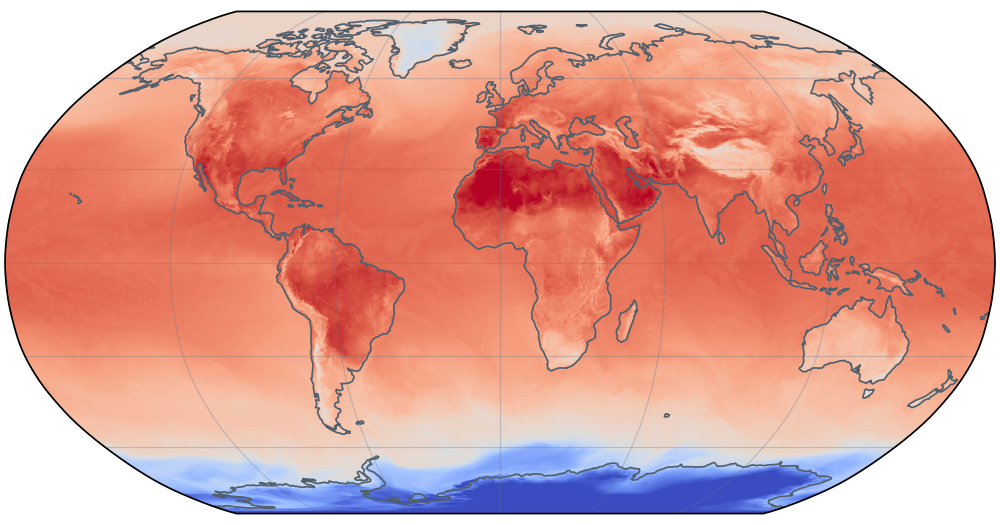
\includegraphics[width=3.35cm]{figures/era5_2t_18.png}};
\node[labeltext] (targetlabel) at (15.05,4.5) {$\mathbf{Y}_c$ at $t+\tau$};

% One-token close-up. A selected channel set is fitted separately per j.
\draw[rounded corners=3pt,draw=black!20,fill=black!1] (.15,.12) rectangle (16.95,3.12);
\node[anchor=west,font=\bfseries,text=probeOrange] at (.4,2.85) {One spatial token, one latent level};
\node[labeltext] at (2.1,2.25) {$D$ activation channels};
\foreach \i in {0,...,11} {
  \filldraw[fill=black!9,draw=white,line width=.6pt] ({.55+.26*\i},1.15) rectangle ++(.26,.55);
}
\foreach \i in {1,4,8} {
  \filldraw[fill=probeOrange!65,draw=white,line width=.6pt] ({.55+.26*\i},1.15) rectangle ++(.26,.55);
}
\node[labeltext,font=\scriptsize] at (2.1,.72) {Select $k$, then standardize\\Separately for each position $j$};
\node[box,draw=probeBlue!70,fill=probeBlue!6,minimum width=3.4cm,minimum height=.85cm] (readout) at (6.5,1.42)
  {\textbf{Linear readouts}\\$\mathbf{w}_{c,j}^{\top}\mathbf{h}_{c,j}(n)+\beta_{c,j}$};
\node[labeltext,font=\scriptsize] at (6.5,.55) {One readout per patch cell\\Weights shared across spatial tokens};
\draw[flow,shorten <=1mm,shorten >=1mm] (3.67,1.42) -- (readout.west);
\draw[flow,shorten <=1mm,shorten >=1mm] (readout.east) -- (9.7,1.42);
\node[labeltext] at (10.45,2.55) {Predicted ERA5 patch};
\foreach \i in {0,...,3} {
  \foreach \j in {0,...,3} {
    \filldraw[fill=probeBlue!9,draw=white,line width=.7pt] ({9.7+.36*\i},{.72+.36*\j}) rectangle ++(.36,.36);
  }
}
\draw[draw=probeBlue!65,line width=.5pt] (9.7,.72) rectangle (11.14,2.16);
\filldraw[fill=probeOrange!45,draw=probeOrange,line width=.8pt] (10.06,1.44) rectangle ++(.36,.36);
\node[font=\scriptsize] at (10.24,1.62) {$j$};
\node[labeltext,font=\scriptsize] at (10.45,.4) {$\widehat{\mathbf{Y}}_c(n,j)$, schematic};
\node[box,minimum width=3.1cm,minimum height=.85cm] (eval) at (15.05,1.42)
  {\textbf{Compare with ERA5}\\MAE, RMSE, spatial $\rho$};
\draw[flow,shorten <=1mm,shorten >=1mm] (11.14,1.42) -- (eval.west);
\draw[flow,shorten <=2mm,shorten >=1mm] (targetlabel.south) -- (eval.north);
\end{tikzpicture}
